% !TEX TS-program = xelatex
% !TEX encoding = UTF-8 Unicode

% Tennessee Technological University
% ME4020 - Fall 2022
% Tristan Hill - November 09, 2022
% Electric Motor Selection 

\documentclass[fleqn]{beamer} % for presentation (has nav buttons at bottom)

% custom preamble
\usepackage{/home/thill/courses/machine_design/machine_design_lecture}

\newcommand{\MNUM}{1\hspace{2mm}} % Module number
\newcommand{\TNUM}{1\hspace{2mm}} % Topic number 
\newcommand{\moduletitle}{Power Screws and Bolted Connections} 
\newcommand{\lecturetitle}{Motor Selection} 

\newcommand{\sectiontitleI}{Classification of Electric Motors}
\newcommand{\sectiontitleII}{Open Loop and Closed Loop Control}
\newcommand{\sectiontitleIII}{Motor Torque-Speed Curves}
\newcommand{\sectiontitleIV}{Analysis and Selection}

\author{ME4020 - Applied Machine Design}
\title{\GD \moduletitle}
\date{Mechanical Engineering\vspc Tennessee Technological University}

\begin{document}

\lstset{language=MATLAB,basicstyle=\ttfamily\small,showstringspaces=false}

\frame{\titlepage \center\begin{framed}\Large \textbf{\lecturetitle}\end{framed} \vspace{5mm}}

% Section 0 - Outline
\frame{
	
	\large \textbf{\lecturetitle} \vspace{3mm}\\
	
	\begin{itemize}
	
		\item \hyperlink{sectionI}{\color{black}\sectiontitleI}	\vspace{3mm} % Section I
		\item \hyperlink{sectionII}{\color{black}\sectiontitleII}	\vspace{3mm} % Section II
		\item \hyperlink{sectionIII}{\color{black}\sectiontitleIII}	\vspace{3mm} %Section III
		\item \hyperlink{sectionIV}{\color{black}\sectiontitleIV}	\vspace{3mm} %Section IV
		%\item \hyperlink{sectionV}{\color{black}\sectiontitleV} %Section IV	
	
	\end{itemize}

}

% Section I
\section{\sectiontitleI}

	% Section I - Frame I
	
	

		\begin{frame}[label=sectionI] \small
			\frametitle{\sectiontitleI}	
	
			\begin{multicols}{2}
				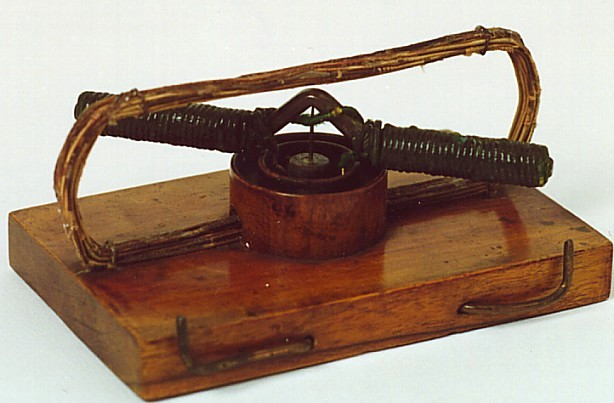
\includegraphics[scale=0.25]{images/Jedlik_motor.jpeg}	
				\href{https://en.wikipedia.org/wiki/Electric_motor}{Jedlik's Electromagnetic Self-Rotor}

				\includegraphics[scale=0.15]{images/MIT-mini-cheetah-01_0.jpg}
				\href{https://news.mit.edu/2019/mit-mini-cheetah-first-four-legged-robot-to-backflip-0304}{MIT Mini Cheetah}
			\end{multicols}

		\end{frame}


	

	% Section I - Frame II
	\begin{frame}[label=sectionI] \small
		\frametitle{\sectiontitleI}	
		
		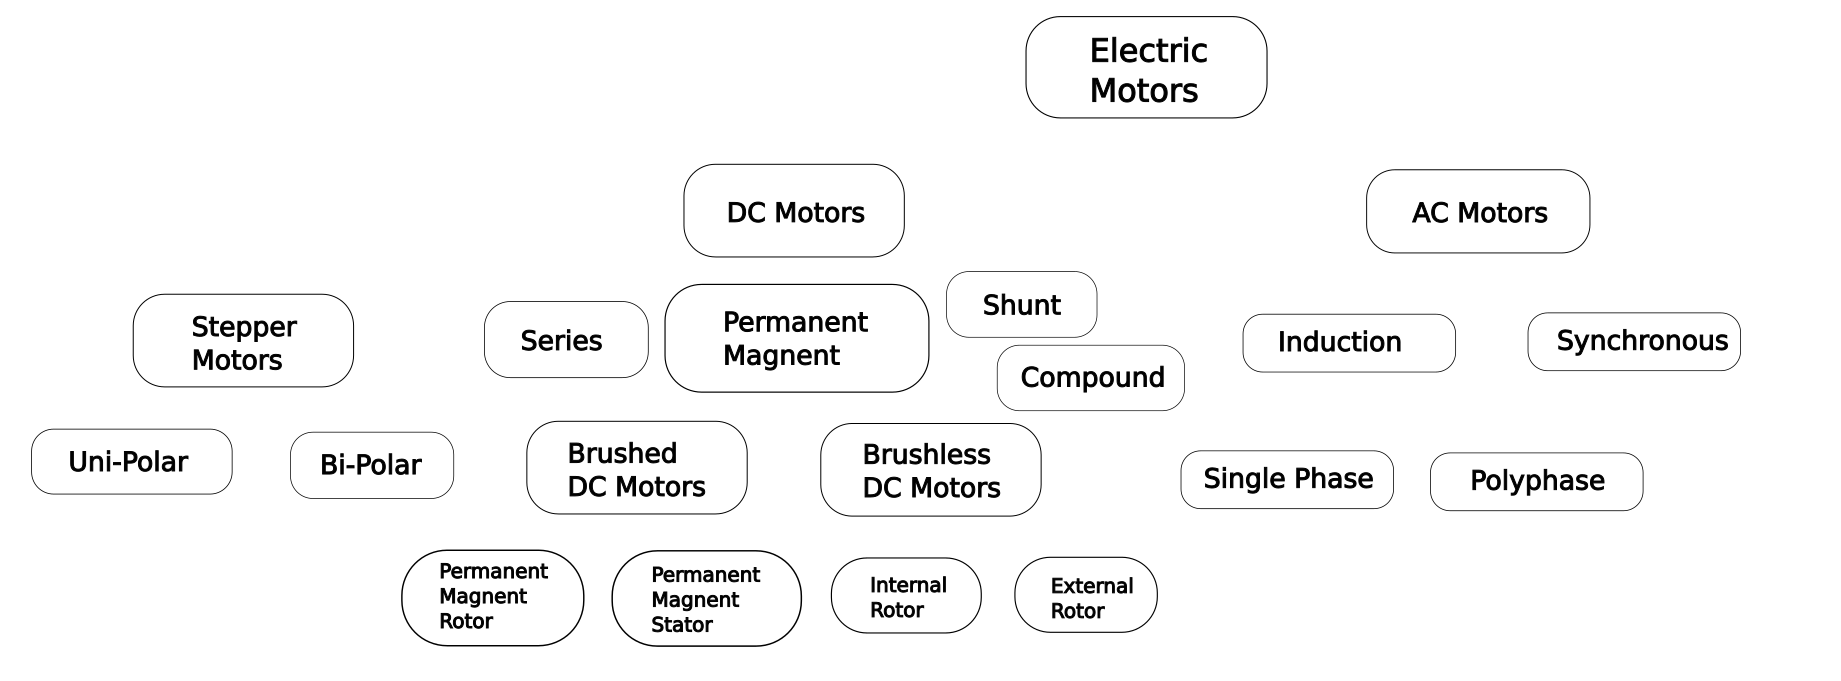
\includegraphics[scale=0.25]{images/classes_of_motors.png}

	\end{frame}


	% Section I - Frame III
	\begin{frame}[label=sectionI] \small
		\frametitle{\sectiontitleI}	
		
		Common Electric Motor Types

		\begin{tabular}{|c|c|c|c|} 
			--- Type --- & --- Example --- & --- Application --- \\ \hline  
			& 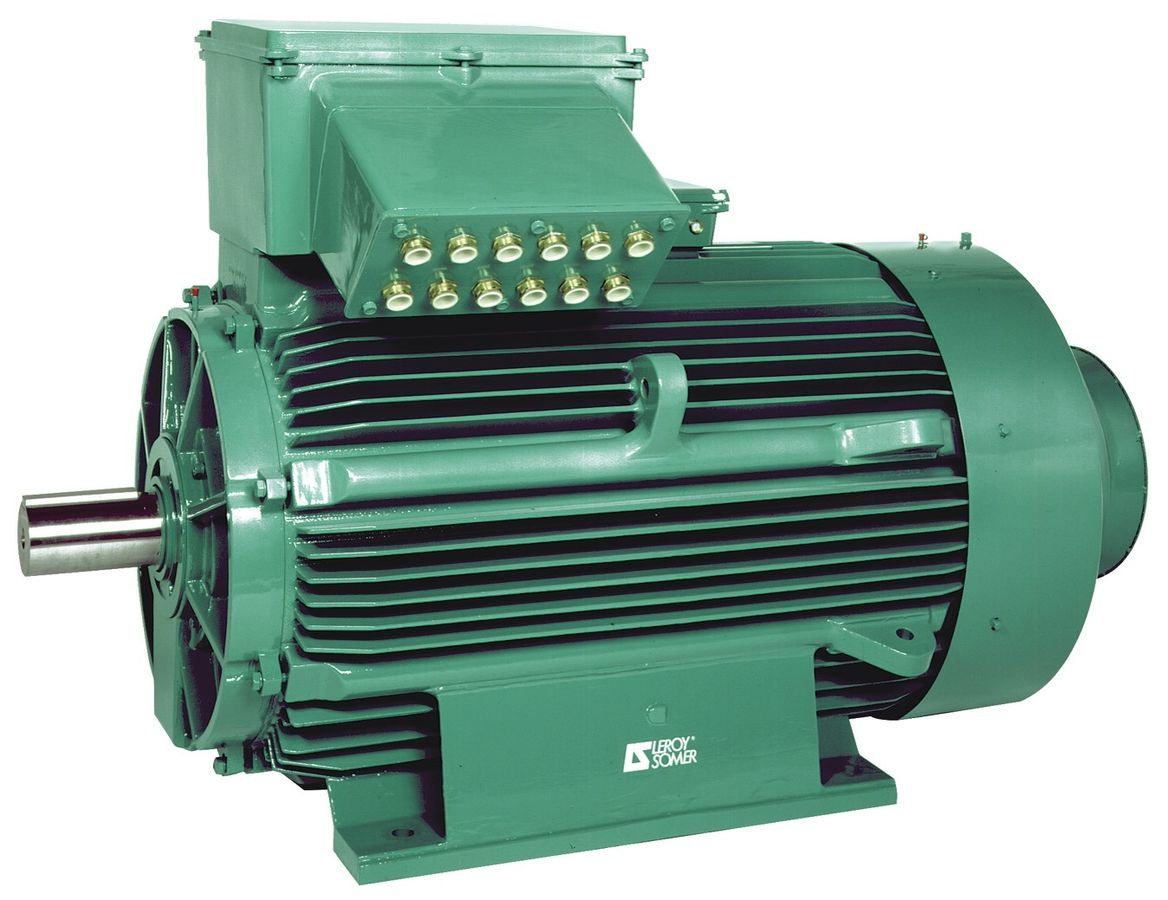
\includegraphics[scale=.05]{images/Ac-elektromotor-robuster-asynchronmotor.jpeg} & \\ \hline                  % AC Motor
			& 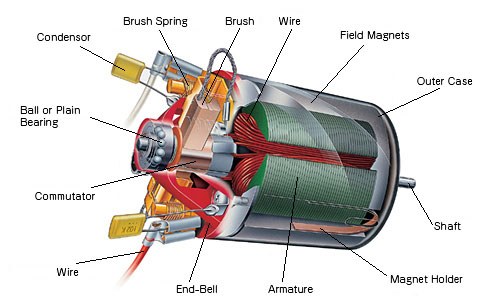
\includegraphics[scale=.29]{images/brushed_dcmotor.jpg} & \\ \hline                  % Brushed DC Motor 
 
		\end{tabular}

	\end{frame}

		% Section I - Frame IV
	\begin{frame}[label=sectionI] \small
		\frametitle{\sectiontitleI}	
		
		Common Electric Motor Types

		\begin{tabular}{|c|c|c|c|} 
			--- Type --- & --- Example --- & --- Applications --- \\ \hline  
			& 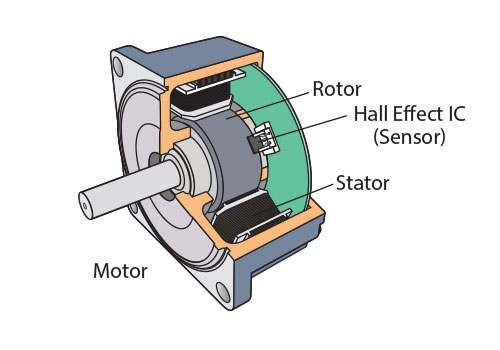
\includegraphics[scale=.2]{images/brushless-dc-motor-structure-and-control.jpg} & \\ \hline                % Brushless DC Motor
			& 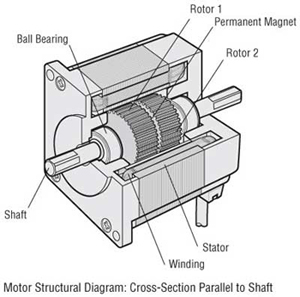
\includegraphics[scale=.2]{images/stepper-motor-structural-diagram.jpg} & \\ \hline                    % Stepper Motor  
		\end{tabular}

	\end{frame}



	% Section I - Frame V
	\begin{frame}[label=sectionI] \small
		\frametitle{\sectiontitleI}	
		
		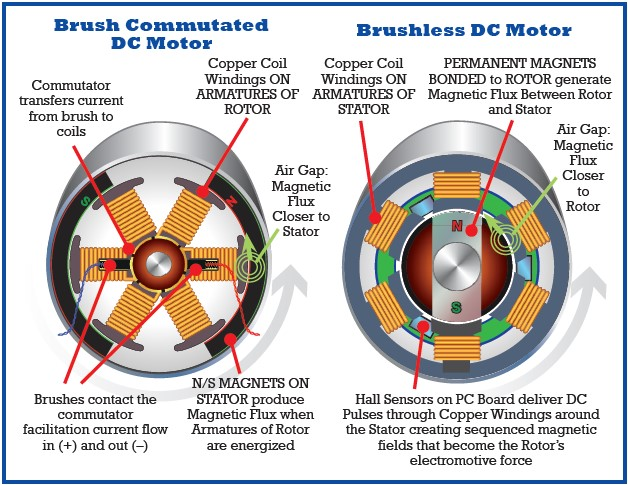
\includegraphics[scale=0.5]{images/brushed_brushless.jpg}

	\end{frame}


% Section II
\section{\sectiontitleII}	

	% Section II - Frame I
	\begin{frame} \small
		\frametitle{\sectiontitleII}

		Open Loop vs Closed Loop Control
		\begin{itemize}
			\item Open Loop Control
			\item Bang-Bang Control
			\item Armature Control
			\item Position Control
			\item Velocity Control
		\end{itemize}

	\end{frame}

	% Section II - Frame II
	\begin{frame} \small
		\frametitle{\sectiontitleII}

		Feedback Controlled Brushed DC Electric Motor

		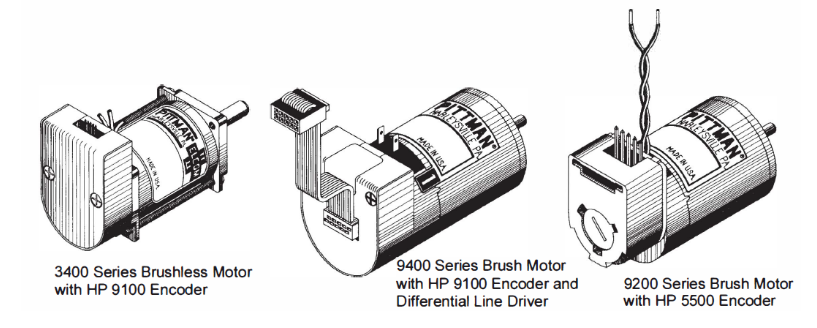
\includegraphics[scale=0.25]{images/pittman_encoder_01.png} \\
	
		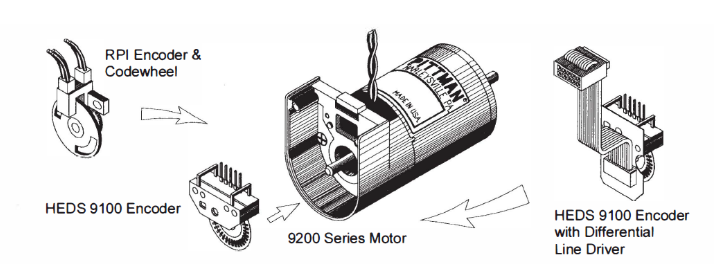
\includegraphics[scale=0.25]{images/pittman_encoder_02.png}	

	\end{frame}

	% Section II - Frame II
	\begin{frame} \small
		\frametitle{\sectiontitleII}

		Feedback Controlled Brushless DC Electric Motor \\

		Modern Case Study: Universl Robotics - Arm Joint

		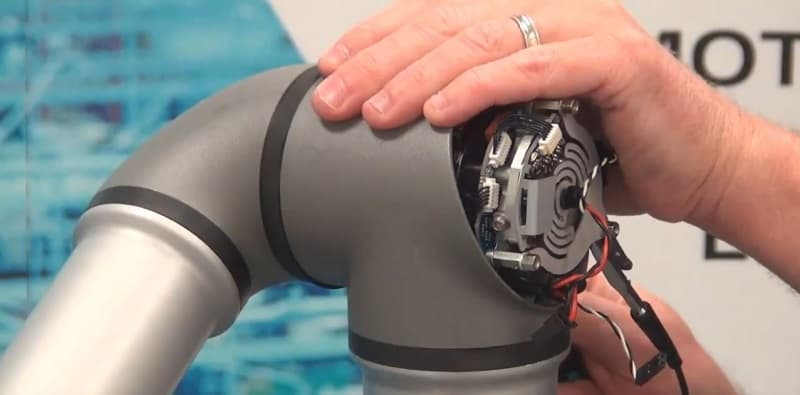
\includegraphics[scale=.25]{images/UR3-Joint-Replacement.jpg}
	
	\end{frame}

		% Section I - Frame III
	\begin{frame} \small
		\frametitle{\sectiontitleII}

		Applications:
		\begin{itemize}
			\item  
			\item
			\item
        \end{itemize}

        \begin{multicols}{2}
		\underline{Pros}
		\begin{itemize}
		\item
		\item
		\item
		\end{itemize}
		\underline{Cons}
		\begin{itemize}
		\item 
		\item
		\item
		\end{itemize}
		\end{multicols}

	\end{frame}

	


	% Section II - Frame I
	\begin{frame}[label=sectionI] \small
		\frametitle{\sectiontitleII}

	\end{frame}

% Section III
\section{\sectiontitleIII}	

	% Section III - Frame I
	\begin{frame}[label=sectionIII] \small
		\frametitle{\sectiontitleIII}
	 		

		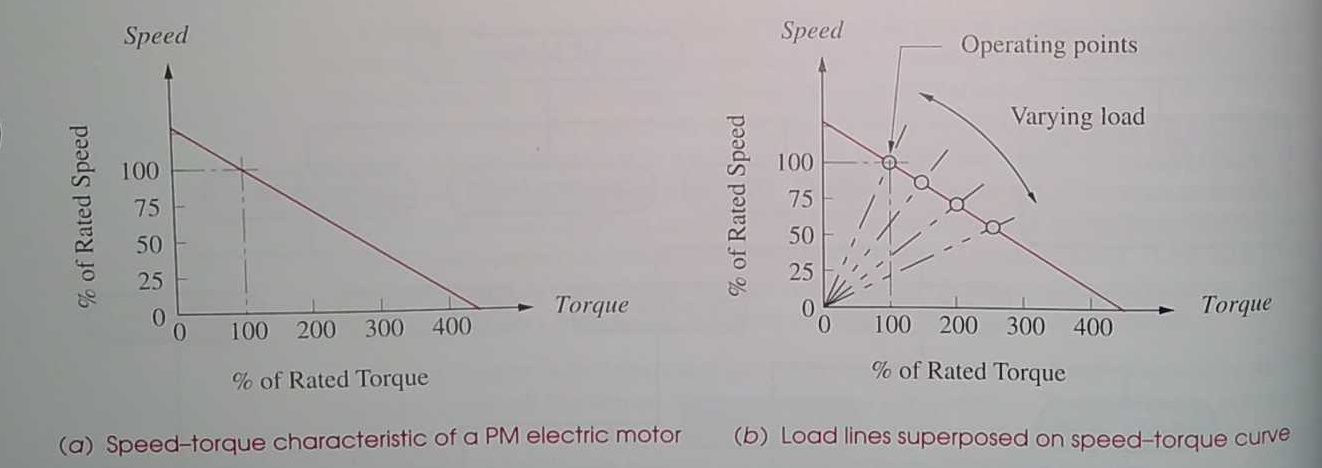
\includegraphics[scale=.25]{images/torque_speed_permanent_magnet.png}

	        
		\end{frame}  

		% Section III - Frame I
	\begin{frame}[label=sectionIII] \small
		\frametitle{\sectiontitleIII}
	 		

		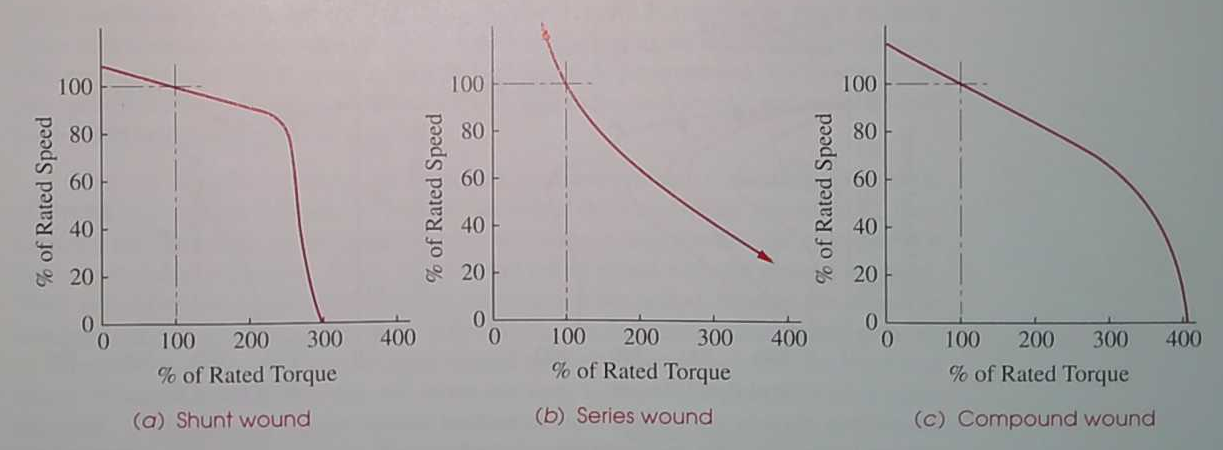
\includegraphics[scale=.25]{images/torque_speed_various.png}

	        
		\end{frame}  
	
% Section IV	
\section{\sectiontitleIV}	
	% Section IV - Frame I
	    \begin{frame}[label=sectionIV] \small
		\frametitle{\sectiontitleIV}    
  
  		\href{https://www.haydonkerkpittman.com/products/motors/brushed-dc-motors/dc054b}{Haydon Kerk Pittman Ametek - Brushed DC }

  		\href{https://www.haydonkerkpittman.com/products/motors/brushless-dc-motors/ec057b}{Haydon Kerk Pittman Ametek - Brushless DC }



		\end{frame}
		
\end{document}